\chapter{Optimizing Neural Networks}
\label{sec-nn-details}

\subsection{Strategies towards adaptive step-size}\label{adaptive-step-size-appendix}
\subsubsection{Running averages}
\index{adaptive step size!running average}
We'll start by looking at the notion of a {\em running average}.  It's
a computational strategy for estimating a possibly weighted average of
a sequence  of data.  Let our data sequence be $c_1, c_2, \ldots$;
then we define a sequence of running average values, $C_0, C_1, C_2,
  \ldots$ using the equations
\begin{align*}
  C_0 & = 0                                       \\
  C_t & =  \gamma_t C_{t-1} +  (1 - \gamma_t) c_t
\end{align*}
where $\gamma_t \in (0, 1)$.  If $\gamma_t$ is a constant, then this
is a {\em  moving} average, in which
\begin{align*}
  C_T & = \gamma C_{T-1} + (1  - \gamma) c_T                                  \\
      & = \gamma (\gamma C_{T-2} + (1  - \gamma) c_{T-1}) + (1  - \gamma) c_T \\
      & = \sum_{t = 1}^T \gamma^{T-t}(1 - \gamma) c_t
\end{align*}
So, you can see that inputs $c_t$ closer to the end of the sequence $T$
have  more effect on $C_T$ than early inputs.

If, instead, we set $\gamma_t = (t - 1)  / t$, then we get the actual
average.
\question{
  Prove to yourself that the previous assertion holds.
}
% \begin{align*}
% A_1 &= a_1\\
% A_2 &= \frac{1}{2}A_1 + \frac{1}{2}a_2 = \frac{1}{2}(a_1 + a_2)\\
% A_3 &= \frac{2}{3}A_2 + \frac{1}{3}a_3 = \frac{2}{3} \cdot \frac{1}{2}(a_1 + a_2) + \frac{1}{3}a_3 = \frac{1}{3}(a_1 + a_2 + a_3)
% \end{align*}

\subsubsection{Momentum} \index{adaptive step size!momentum}
Now, we can use methods that are a bit like running averages to
describe strategies for computing $\eta$.
The simplest method is {\em momentum}, in  which we try to ``average'' recent
gradient updates,  so that if they have been bouncing back and forth
in some direction, we take out that component of the motion.  For
momentum, we have
\begin{align*}
  V_0 & = 0                                         \\
  V_t & = \gamma V_{t-1} + \eta \nabla_W J(W_{t-1}) \\
  W_t & = W_{t-1} - V_t
\end{align*}
This doesn't quite look like an adaptive step size.  But what we can
see is that, if we let $\eta = \eta'(1 - \gamma)$, then the rule looks exactly like doing an update with
step size $\eta'$ on a moving average of the gradients with parameter
$\gamma$:
\begin{align*}
  M_0 & = 0                                                 \\
  M_t & = \gamma M_{t-1} + (1 - \gamma) \nabla_W J(W_{t-1}) \\
  W_t & = W_{t-1} - \eta' M_t
\end{align*}
\question{Prove to yourself that these formulations are equivalent.}


We will find that $V_t$ will be bigger in dimensions that consistently
have the same sign for $\nabla_{W}$ and smaller for those that
don't.   Of course we now have {\em two}  parameters  to set ($\eta$
and $\gamma$), but the
hope is  that the algorithm will perform better overall, so it will be
worth trying to find good values for them.  Often $\gamma$ is  set to
be something like $0.9$.
\begin{examplebox}
  \begin{center}
    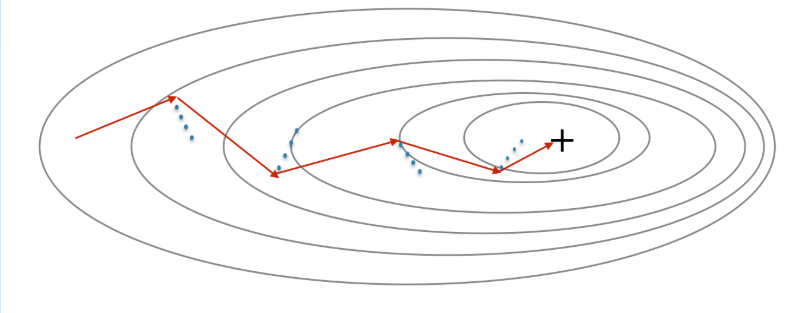
\includegraphics[scale=0.7]{figures/momentum.png}
  \end{center}
  The red arrows show the update after each successive step of
  mini-batch gradient descent with momentum.  The blue points show the
  direction of the gradient with respect to the mini-batch at each step.
  Momentum smooths the path taken towards the local minimum and leads to
  faster convergence.
\end{examplebox}
\question{If you set $\gamma = 0.1$, would momentum have more of an
  effect or less of an effect than if you set it to $0.9$?
}

\subsubsection{Adadelta}\index{adaptive step size!adadelta}
Another useful idea is this:  we would like to take larger steps in
parts of the space where $J(W)$ is nearly flat (because there's no risk of
taking too big a step due to the gradient being large) and smaller
steps when it is steep.  We'll apply this idea to each weight
independently, and end up with a method called {\em adadelta}, which
is a variant on {\em adagrad} (for
adaptive gradient).   Even though our weights are indexed by layer,
input unit and output unit,  for simplicity here,  just let $W_j$ be
any weight in the network (we will do the same thing for all of
them).
\begin{align*}
  g_{t,j} & = \nabla_W J(W_{t-1})_j                                      \\
  G_{t,j} & = \gamma G_{t - 1,j} + (1 - \gamma)g_{t,j}^2                 \\
  W_{t,j} & = W_{t-1, j} - \frac{\eta}{\sqrt{G_{t,j} + \epsilon}}g_{t,j}
\end{align*}
The sequence $G_{t,j}$ is a moving average of the  square of the
$j$th component of the gradient.  We square it in order to be
insensitive to the sign---we want to know whether the magnitude is big
or small.  Then, we perform a gradient update to weight $j$, but
divide the step  size by $\sqrt{G_{t,j} + \epsilon}$, which is larger
when the surface is steeper in direction $j$ at point $W_{t-1}$ in
weight space;  this means that the step size will be smaller when it's
steep and  larger when it's flat.

\subsubsection{Adam}\index{adaptive step size!adam}

Adam has become the default method of managing step sizes in neural
networks\note{Although,  interestingly, it may actually violate the
convergence conditions of {\sc sgd}: {\scriptsize\tt
arxiv.org/abs/1705.08292}}.   It combines the ideas  of
momentum and adadelta.  We start by writing moving averages of the
gradient and squared gradient, which reflect estimates of the mean and
variance of the gradient for weight $j$:
\begin{align*}
  g_{t,j} & = \nabla_W J(W_{t-1})_j                      \\
  m_{t,j} & = B_1m_{t - 1,j} + (1 - B_1)g_{t,j}          \\
  v_{t,j} & = B_2v_{t - 1,j} + (1 - B_2)g_{t,j}^2  \;\;.
\end{align*}

A problem with these estimates is that, if we initialize $m_0 = v_0 = 0$,
they will always be biased (slightly too small).  So we will correct
for that bias  by defining
\begin{align*}
  \hat{m}_{t,j} & = \frac{m_{t,j}}{1 - B^t_1}                     \\
  \hat{v}_{t,j} & = \frac{v_{t,j}}{1 - B^t_2}                     \\
  W_{t,j}       & = W_{t-1,j} - \frac{\eta}{\sqrt{\hat{v}_{t,j} +
      \epsilon}}\hat{m}_{t,j} \;\;.
\end{align*}
Note that $B^t_1$ is $B_1$ raised to the power $t$, and likewise for
$B^t_2$.  To justify these corrections, note that if we were to expand $m_{t,j}$
in terms of $m_{0,j}$ and $g_{0,j}, g_{1,j}, \dots, g_{t,j}$ the coefficients would
sum to $1$.  However, the coefficient behind $m_{0,j}$ is $B_1^t$ and since
$m_{0,j} = 0$, the sum of coefficients of non-zero terms is $1 - B_1^t$, hence
the correction.  The same justification holds for $v_{t,j}$.

Now, our update for weight $j$ has a step size that takes the
steepness into account, as in adadelta, but also tends to move in the
same direction, as in momentum.  The authors of this method propose
setting $B_1 = 0.9, B_2 = 0.999, \epsilon = 10^{-8}$.  Although we now
have even more parameters, Adam is not highly sensitive to their values
(small changes do not have a huge effect on the result).
\question{Define $\hat{m_j}$ directly as a moving average of
  $g_{t,j}$.  What is the decay ($\gamma$ parameter)?
}
Even though we now have a step-size for each weight, and we have to
update various quantities on each iteration of gradient descent, it's
relatively easy to implement by maintaining a matrix for each quantity
($ m^{\ell}_t, v^{\ell}_t, g^{\ell}_t, {g^{2}_t}^{\ell} $) in each
layer of the network.





% 

\subsection{Batch Normalization Details}\label{batch-norm-appendix}

Let's think of the batch-norm layer as taking $Z^l$ as input and
producing an output $\widehat{Z}^l$ as output.  But now, instead of
thinking of $Z^l$ as an $n^l \times 1$ vector, we have to explicitly
think about handling a mini-batch of data of size $K$, all at once, so
$Z^l$ will be $n^l \times K$, and so will the output $\widehat{Z}^l$.

Our first step will be to compute the {\em batchwise} mean and
standard deviation.  Let $\mu^l$ be the $n^l \times 1$ vector where
\[\mu^l_i = \frac{1}{K} \sum_{j = 1}^K Z^l_{ij}\;\;,\]
and let $\sigma^l$ be the $n^l \times 1$ vector where
\[\sigma^l_i = \sqrt{\frac{1}{K} \sum_{j = 1}^K (Z^l_{ij} - \mu_i)^2}\;\;.\]

The basic normalized version of our data would be a matrix,
element $(i, j)$ of which is
\[\overline{Z}^l_{ij} = \frac{Z^l_{ij} - \mu^l_i}{\sigma^l_i + \epsilon}\;\;,\]
where $\epsilon$ is a very small constant to guard against division by
zero.
However, if we let these be our $\widehat{Z}^l$ values, we really are
forcing something too strong on our data---our goal was to normalize
across the data batch, but not necessarily force the output values to
have exactly mean 0 and standard deviation 1.  So, we will give the
layer the ``opportunity'' to shift and scale the outputs by adding new
weights to the layer.  These weights are $G^l$ and $B^l$, each of
which is an $n^l \times 1$ vector.  Using the weights, we define the
final output to be
\[\widehat{Z}^l_{ij} = G^l_i \overline{Z}^l_{ij} + B^l_i\;\;.\]
That's the forward pass.  Whew!

Now, for the backward pass, we have to do two things:  given
$\partial L / \partial \widehat{Z}^l$,
\begin{itemize}
  \item Compute $\partial L / \partial Z^l$ for back-propagation, and
  \item Compute $\partial L / \partial G^l$ and $\partial L / \partial
          B^l$ for gradient updates of the weights in this layer.
\end{itemize}

Schematically\note{For simplicity we will drop the reference to the layer $l$ in the rest of the derivation}
\[\frac{\partial L}{\partial B} = \frac{\partial L}{\partial
    \widehat{Z}}\frac{\partial \widehat{Z}}{\partial B}\;\;.\]
It's hard to think about these derivatives in matrix terms, so we'll
see how it works for the components.
$B_i$ contributes to $\widehat{Z}_{ij}$ for all data points $j$ in the
batch.  So
\begin{align*}
  \frac{\partial L}{\partial B_i} & =
  \sum_j \frac{\partial L}{\partial \widehat{Z}_{ij}}
  \frac{\partial \widehat{Z}_{ij}}{\partial B_i}                                               \\
                                  & = \sum_j \frac{\partial L}{\partial \widehat{Z}_{ij}}\;\;,
\end{align*}
Similarly, $G_i$ contributes to $\widehat{Z}_{ij}$ for all data points
$j$ in the batch.  So
\begin{align*}
  \frac{\partial L}{\partial G_i} & =
  \sum_j \frac{\partial L}{\partial \widehat{Z}_{ij}}
  \frac{\partial \widehat{Z}_{ij}}{\partial G_i}                                                                  \\
                                  & =  \sum_j \frac{\partial L}{\partial \widehat{Z}_{ij}} \overline{Z}_{ij}\;\;.
\end{align*}
Now, let's figure out how to do backprop.  We can start schematically:
\[\frac{\partial L}{\partial Z} = \frac{\partial L}{\partial \widehat{Z}}
  \frac{\partial \widehat{Z}}{\partial Z}\;\;.\]
And because dependencies only exist across the batch, but not across
the unit outputs,
\[\frac{\partial L}{\partial Z_{ij}} =
  \sum_{k=1}^K\frac{\partial L}{\partial \widehat{Z}_{ik}}
  \frac{\partial \widehat{Z}_{ik}}{\partial Z_{ij}}\;\;.\]
The next step is to note that
\begin{align*}
  \frac{\partial \widehat{Z}_{ik}}{\partial Z_{ij}} & =
  \frac{\partial \widehat{Z}_{ik}}{\partial \overline{Z}_{ik}}
  \frac{\partial \overline{Z}_{ik}}{\partial Z_{ij}}                                                                \\
                                                    & = G_i \frac{\partial \overline{Z}_{ik}}{\partial Z_{ij}}\;\;.
\end{align*}
And now that
\[
  \frac{\partial \overline{Z}_{ik}}{\partial Z_{ij}}  =
  \left(\delta_{jk} - \frac{\partial \mu_i}{\partial Z_{ij}}\right) \frac{1}{\sigma_i} -
  \frac{Z_{ik} - \mu_i}{\sigma_i^2} \frac{\partial \sigma_i}{\partial Z_{ij}} \;\;,
\]
where $\delta_{jk} = 1$ if $j = k$ and $\delta_{jk} = 0$ otherwise.
Getting close!  We need two more small parts:
\begin{align*}
  \frac{\partial \mu_i}{\partial Z_{ij}}    & = \frac{1}{K} \;, \\
  \frac{\partial \sigma_i}{\partial Z_{ij}} & =
  \frac{Z_{ij} - \mu_i}{K \sigma_i}\;\;.
\end{align*}
Putting the whole crazy thing together, we get
\[\frac{\partial L}{\partial Z_{ij}} =
  \sum_{k=1}^K\frac{\partial L}{\partial \widehat{Z}_{ik}}
  G_i\frac{1}{K \sigma_i}\left(\delta_{jk}K-1 - \frac{(Z_{ik} - \mu_i)(Z_{ij} - \mu_i)}{\sigma_i^2}
  \right)\;\;.
\]